% TODO

% Meet before pres 9:20 - 9:30 ish

% why do we include the other d orbitals? why not just 2
% because they influnece the electronic states near fermi level, see eigenvector, basis states etc
% single layer rotation

% talk about Perturbation theory - energy splitting - can see this with simple coupling model!
% flatness of bands
% = interesting stuff

% moire patterns, why?
% can't gaurantee periodicity

% dz2 interaction may only be periodic in superlattice
% in which case hamiltonian is only true in superlattice periodicity

% large brillouin one means more states

\documentclass[9pt]{beamer}

\usetheme{default}

\usepackage{graphicx}
\usepackage{booktabs}
\usepackage{array}
\usepackage{paralist}
\usepackage{verbatim}
\usepackage{subfig}
\usepackage{amsmath}
\usepackage[none]{hyphenat}

%title page
\title{Twisted bilayer NbSe$_2$}
\subtitle{Semester 1 presentation}
\author{Conan Birkett}
\institute{University of Bath department of Physics}

\begin{document}

\begin{frame}
  \titlepage
\end{frame}

\begin{frame}{Outline}
  \begin{itemize}
      \item Introduction
      \item Modelling NbSe$_2$
      \item Adding a twist
      \item Constructing a heterostructure
      \item What's next? - Layer coupling and perturbation theory
      \item References
  \end{itemize}
\end{frame}

\begin{frame}{Introduction}
  \begin{itemize}
    \item In 2018 Cao Y. et al realised unconventional superconductivity in 'magic-angle' twisted bilayer graphene$^{[1]}$, previously predicted in 2011 by R. Bistritzer and A. MacDonald$^{[2]}$.

    \item This has prompted a wave of research in the newly dubbed field of 'Twistronics', the study of the electronic properties of twisted Van der Waals heterostructures$^{[3][4]}$.

    \item Our project examines a Van der Waals heterostructure of two 2H-NbSe$_2$ layers. Our objective is to determine if a magic angle exists in this material, and if so to offer an interpretation of the resulting electronic band structure.
  \end{itemize}
\end{frame}

\begin{frame}{Tight binding model with spin orbit coupling}{Modelling NbSe$_2$}
  \begin{itemize}
    \item For our model of NbSe$_2$ we employ a multi-orbital tight binding model from R. Habara and K. Wakabayashi $^{[5]}$.

    \item It uses the $d_{z^2}$, $d_{xy}$ and $d_{x^2-y^2}$ orbitals of Nb atoms up to third nearest neighbor sites with spin up and down as a basis set to describe the electronic states of the NbSe$_2$ monolayer near the Fermi level.

    \item{The eigenvalue equation for the TBM is
      \begin{equation}
        \label{TBM_evalue_eqn}
        \hat{H}(\boldsymbol{k})\left|u_{n k}\right\rangle=E_{n k}\left|u_{n k}\right\rangle
      \end{equation}

      where $k=\left(k_{x}, k_{y}\right)$ is the wave-number vector, $E_{nk}$ is the eigenvalue and $n = 1,2,\cdots,6$ is the band index.
      }

    \item{The eigenvector is defined as
      \begin{equation}
        \left|u_{n k}\right\rangle=$ $\left(c_{n k, d_{z^{2}}, \uparrow}, c_{n k, d_{x y}, \uparrow}, c_{n k, d_{x^{2}-y^{2}}, \uparrow}, c_{n k, d_{z^{2}}, \downarrow}, c_{n k, d_{x y}, \downarrow}, c_{n k, d_{x^{2}-y^{2}}, \downarrow}\right)^{T}
      \end{equation}

      where $(\cdots)^T$ indicates the transpose of the vector and $c_{nk\tau s}$ is the amplitude at atomic orbital $\tau$ with spin $s$ for the $n$th energy band at $k$.
      }
  \end{itemize}
\end{frame}

\begin{frame}{TBM Nearest Neighbors (NN)}{Modelling NbSe$_2$}

  \begin{figure}
    \centering
    \begin{minipage}{.5\textwidth}
      \centering
      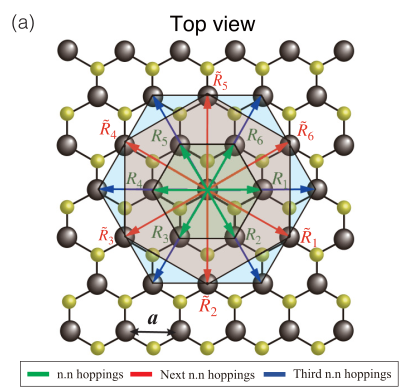
\includegraphics[width=.9\linewidth]{./Habara_NN.png}
    \end{minipage}%
    \begin{minipage}{.5\textwidth}
      \centering
      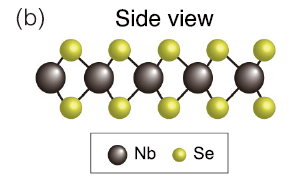
\includegraphics[width=.9\linewidth]{./Habara_side_view.png}
    \end{minipage}
    \captionof{figure}{FIG. 1. (a) and (b) from Habara et al$^{[5]}$ Displaying a top-down view and side view of the structure of monolayer NbSe$_2$ consisting of Nb (black) and Se (yellow) atoms. The first, second and third nearest neighbor sites are shown in green, red and blue respectively. $a$ is the primitive lattice constant.}
  \end{figure}

\end{frame}

\begin{frame}{TBM Hamiltonian}{Modelling NbSe$_2$}
  \begin{itemize}
    \item{The Hamiltonian $\hat{H}(\boldsymbol{k})$ with spin orbit coupling can be written as

      \begin{equation}
        \hat{H}(\boldsymbol{k})=\hat{\sigma}_{0} \otimes \hat{H}_{\mathrm{TNN}}(\boldsymbol{k})+\hat{\sigma}_{z} \otimes \frac{1}{2} \lambda_{\mathrm{SOC}} \hat{L}_{z}
      \end{equation}
      }

    \item{Which is comprised of the tight binding nearest neighbor (NN) Hamiltonian

      \begin{equation}
        \hat{H}_{\mathrm{TNN}}(\boldsymbol{k})=\left(\begin{array}{ccc}
        V_{0} & V_{1} & V_{2} \\
        V_{1}^{*} & V_{11} & V_{12} \\
        V_{2}^{*} & V_{12}^{*} & V_{22}
        \end{array}\right)
      \end{equation}
      }

    \item{And a spin orbit coupling term

      \begin{equation}
        \hat{L}_{z}=\left(\begin{array}{ccc}
        0 & 0 & 0 \\
        0 & 0 & -2 i \\
        0 & 2 i & 0
        \end{array}\right)
      \end{equation}
    }

  \item $\hat{\sigma}_0$ and $\hat{\sigma}_z$ are pauli matrices and $\lambda_{\text{SOC}}=0.0784$ eV is the Ising-type spin orbit coupling parameter. $V_0 \cdots V_{22}$ are functions of $k$ $^{[5]}$.
  \end{itemize}
\end{frame}

\begin{frame}{1st Brillouin zone (BZ)}{Modelling NbSe$_2$}
  \begin{itemize}
    \item The result is a 6 by 6 block-diagonal Hamiltonian that is a function of wavevector $k$.

    \item From our eigenvalue equation \eqref{TBM_evalue_eqn} we can then determine the energy (eigenvalues) of the 6 electronic (eigen-)states at a given point in $k$-space.

    \item Specifically, we can take $k$ from slices in the first brillouin zone along the standard critical points, and even a surface over $k$ space.
  \end{itemize}

  \begin{figure}
    \centering
    \resizebox{4cm}{!}{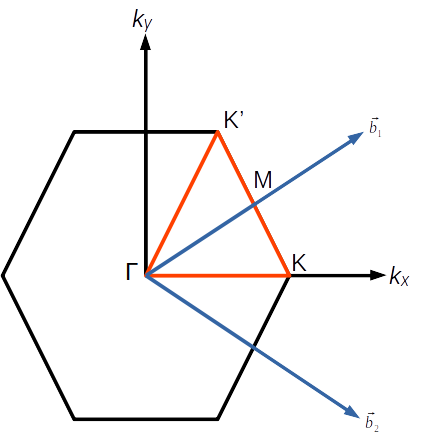
\includegraphics{1st_BZ.png}}
    \caption{The first brillouin zone of the NbSe$_2$ lattice. $\Gamma, K, K' \text{ and } M$ are the standard critical points. $\vec{b_1}, \vec{b_2}$ are the reciprocal lattice vectors, shown in red is the slice $\Gamma \rightarrow K \rightarrow M \rightarrow K' \rightarrow \Gamma$.}
  \end{figure}
\end{frame}

\begin{frame}{Electronic band structure}{Modelling NbSe$_2$}
  \begin{itemize}
    \item As a consequence of Bloch's theorem, the eigenstates and their eigenvalues seen in the 1st brillouin zone repeat throughout the bulk lattice. 

    \item Additionally due to reflectional symmetry the region that fully describes the electronic states can be reduced to the equilateral triangle bounded by $\Gamma \rightarrow K \rightarrow M \rightarrow K' \rightarrow \Gamma$.
  \end{itemize}

  \begin{figure}
  \centering
  \begin{minipage}{.5\textwidth}
    \centering
    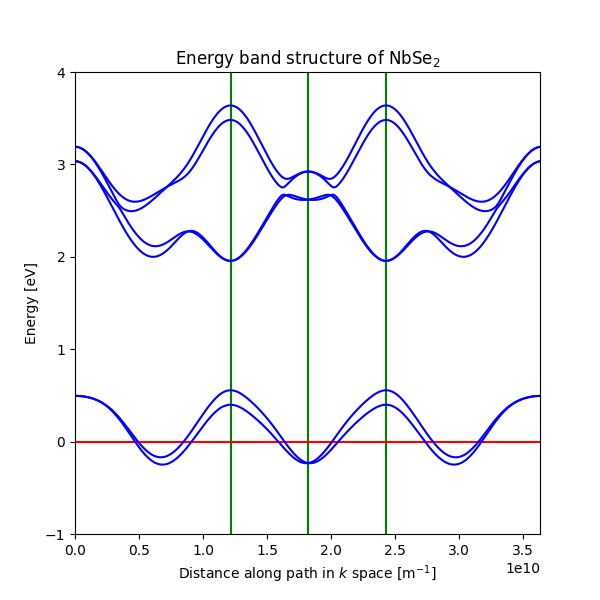
\includegraphics[width=.9\linewidth]{unrotated_evalues.png}
    \captionof{figure}{Energy band structure taken across slice $\Gamma \rightarrow K \rightarrow M \rightarrow K' \rightarrow \Gamma$. Critical points are shown in green and the Fermi level (red) is set to 0 eV.}
  \end{minipage}%
  \begin{minipage}{.5\textwidth}
    \centering
    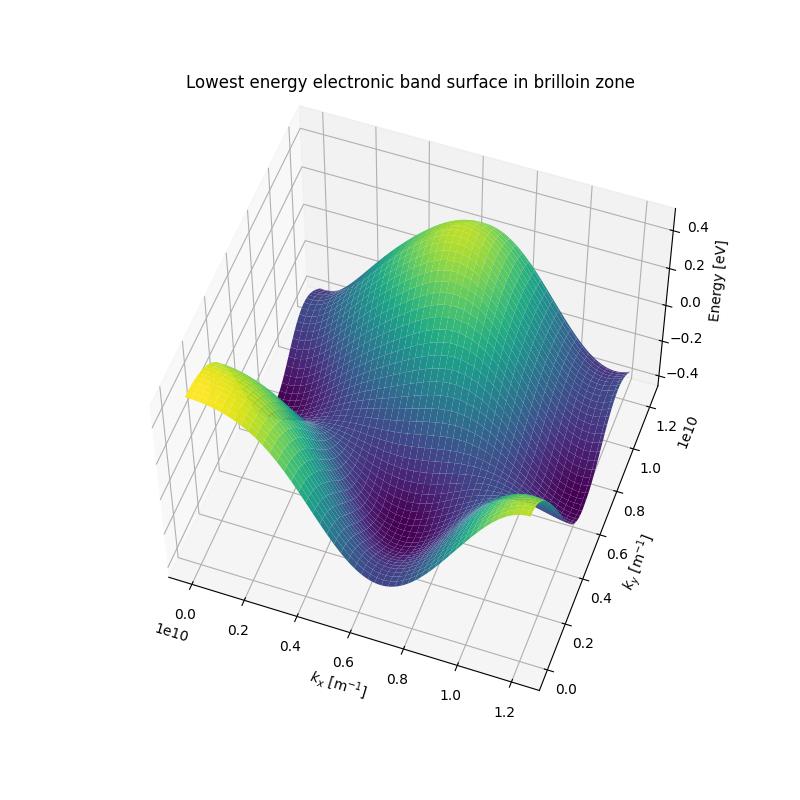
\includegraphics[width=.9\linewidth]{unrotated_surface.png}
    \captionof{figure}{A plot of the surface of the lowest energy state in the same region. The same peaks can be seen at critical points $\Gamma, K, \text{and} K'$.}
  \end{minipage}
  \end{figure}
\end{frame}

\begin{frame}{Habara FIG 1. (d)}{Modelling NbSe$_2$}
  \begin{itemize}
    \item If we instead take the same slice but insead from $M \rightarrow M$ we can retrieve FIG. 1. (d) from Habara et al$^{[5]}$.

    \item In the rest of our analysis we use $\Gamma \rightarrow \Gamma$ as $\Gamma$ is the axis of rotation.
  \end{itemize}

  \begin{figure}
  \centering
  \begin{minipage}{.5\textwidth}
    \centering
    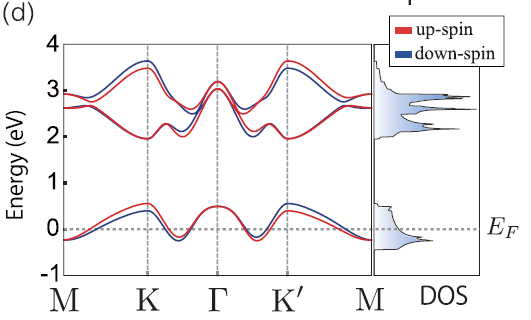
\includegraphics[width=.9\linewidth]{Habara_evalues.png}
  \end{minipage}%
  \begin{minipage}{.5\textwidth}
    \centering
    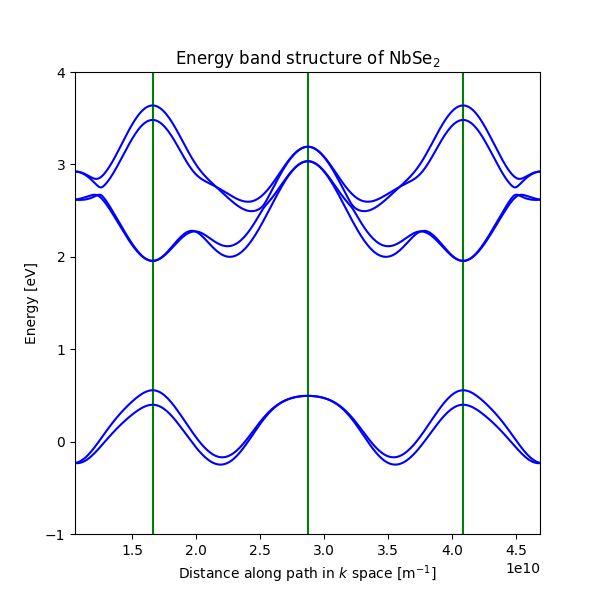
\includegraphics[width=.9\linewidth]{our_Habara_evalues.png}
  \end{minipage}
  \captionof{figure}{Habara et al$^{[5]}$ FIG. 1. (d), Energy band structure and DOS taken across slice $M \rightarrow K' \rightarrow \Gamma \rightarrow K \rightarrow M$. Note they have taken $K$ and $K'$ to have opposite meanings. Our recreation is shown on the right for comparison.}
  \end{figure}
\end{frame}

\begin{frame}{Rotating vectors}{Adding a twist}
  \begin{itemize}
    \item In order to construct a twisted bilayer, we must first figure out how to describe a twisted monolayer.

    \item A simple rotation in primitive lattice vectors $a_1, a_2 -> a_1', a_2'$ corresponds to the same rotation in reciprocal lattice vectors $b_1, b_2 -> b_1', b_2'$.

    \item We can consider this a rotation of the whole coordinate system in $k$ space to coordinates in $(k_x', k_y')$.

    \item The result of this is that in order to describe a vector $\vec{k'}$ in rotated $k$ space (such as $Gamma, K$ etc) in terms of our unrotated coordinate system $(k_x, k_y)$ it has to be rotated \textit{inversely} to the rotation of the layer.
  \end{itemize}
\end{frame}

\begin{frame}{Twisted triangles}{Adding a twist}
  \begin{figure}
  \centering
    \resizebox{6cm}{!}{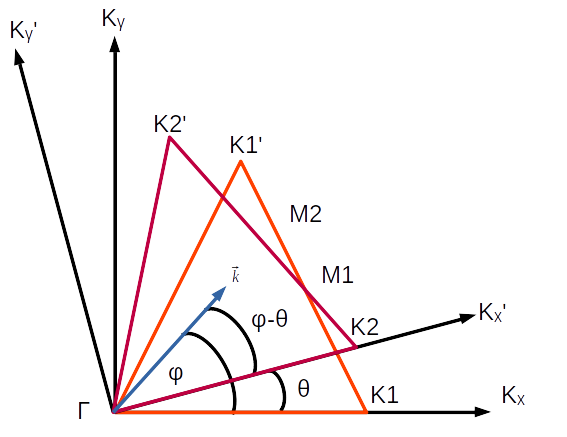
\includegraphics{twisted_triangles.png}}
    \caption{The effect of rotating the layer on the path $\Gamma \rightarrow \Gamma$ and the correction that must be made to $\vec{k}$. Because of the rotation of $(k_x, k_y)$ to $(k_x', k_y')$ by $\theta$, in order for for vector $\vec{k}$ in $k'$ space to be represented in the unrotated $k$ space it must be rotated clockwise by $\theta$.}
  \end{figure}
\end{frame}

\begin{frame}{Two triangle path}{Adding a twist}
  \begin{figure}
  \centering
    \resizebox{6cm}{!}{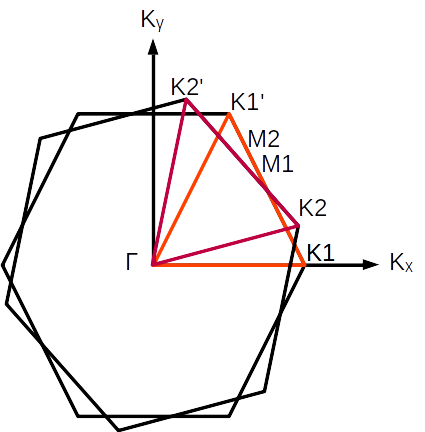
\includegraphics{heterostructure_BZ_path.png}}
    \caption{It is convenient to construct a path consisting of an unrotated path $\Gamma \rightarrow K_1 \rightarrow M_1 \rightarrow K_1' \rightarrow \Gamma$ followed by a rotated path (here at 15$^\circ$)  $\Gamma \rightarrow K_2 \rightarrow M_2 \rightarrow K_2' \rightarrow \Gamma$. This allows us to consider the eigenvalues of a lattice from two perspectives consecutively. We will call this path $\Gamma \rightarrow \Gamma \rightarrow \Gamma$.}
  \end{figure}
\end{frame}

\begin{frame}{Twisted eigenvalues}{Adding a twist}
  \begin{figure}
  \centering
    \resizebox{6cm}{!}{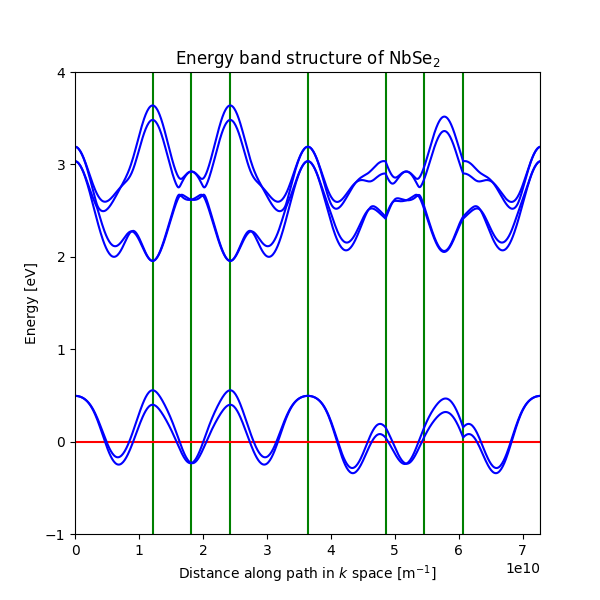
\includegraphics{twisted_evalues_1.png}}
    \caption{Our original plot of eigenvalues of an 'unrotated' layer on the new path $\Gamma \rightarrow \Gamma \rightarrow \Gamma$. There is clearly a substantial effect on the electronic band structure across the rotated portion of the path.}
  \end{figure}
\end{frame}

\begin{frame}{Twisted surface}{Adding a twist}
  \begin{figure}
    \centering
    \resizebox{6cm}{!}{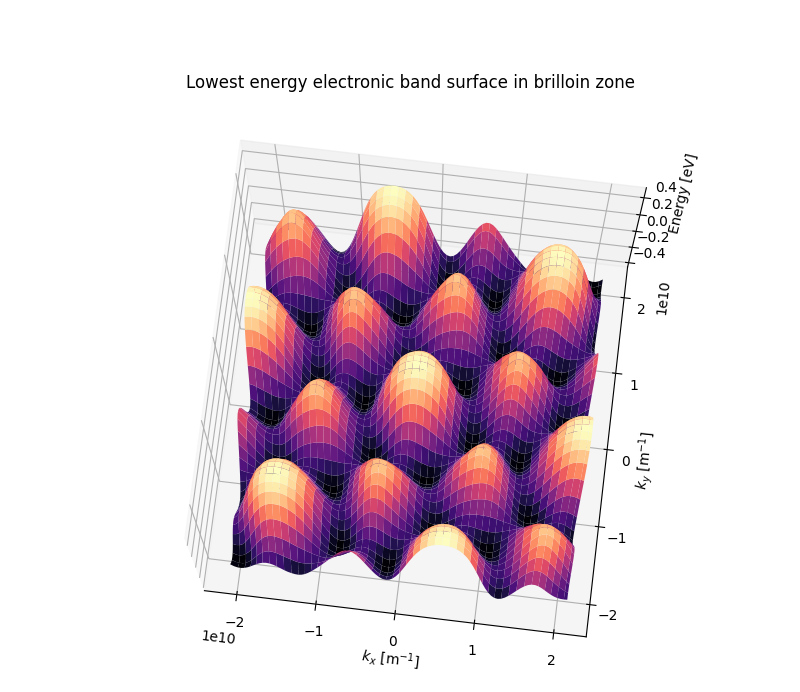
\includegraphics{twisted_mono_surface.png}}
    \caption{A surface of the lowest energy state plotted against unrotated $k_x, k_y$ axes. A twist of 15$^\circ$ is applied to the surface counter clockwise. The plot has been extended to an area encompassing the first brillouin zone to show this more clearly.}
  \end{figure}
\end{frame}

\begin{frame}{Un-twisted eigenvalues}{Adding a twist}
  \begin{figure}
  \centering
    \resizebox{6cm}{!}{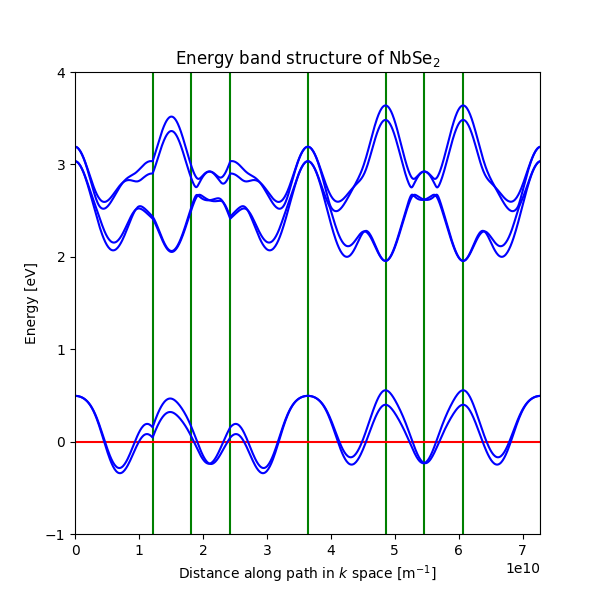
\includegraphics{twisted_evalues_2.png}}
    \caption{The eigenvalues of our 15$^\circ$ twisted lattice on the path $\Gamma \rightarrow \Gamma \rightarrow \Gamma$. It is flipped in the $x$ axis when compared with the eigenvalues of the unrotated lattice.}
  \end{figure}
\end{frame}

\begin{frame}{Heterostructure Hamiltonian}{Constructing a heterostructure}
  \begin{itemize}
    \item Now that we can describe a rotated layer of NbSe$_2$ we can now model two layers at once, with one rotated. A simple model assumes no interaction between states in different layers. 
    \item{We construct a Hamiltonian for the whole system by combining the Hamiltonians of each layer into a 12 by 12 block diagonal matrix

      \begin{equation}
        \hat{H}(\boldsymbol{k})=\left(\begin{array}{cc}
          \hat{H_1}(\boldsymbol{k}) & 0\\
          0 & \hat{H_2}(\boldsymbol{k'})
        \end{array}\right)
      \end{equation}
      
      Where $\hat{H_1}(\boldsymbol{k})$ and $\hat{H_2}(\boldsymbol{k'})$ are the Hamiltonians of the unrotated and rotated layers respectively.
      }
    \item Note that $\hat{H_2}(\boldsymbol{k'})$ is a function of $k'$ which means that an implementation of this matrix of this function must rotate the $k$ input (as described previously) before it is input into $\hat{H}(\boldsymbol{k})$.
  \end{itemize}
\end{frame}

\begin{frame}{Heterostructure eigenvalues}{Constructing a heterostructure}
  \begin{figure}
    \centering
    \resizebox{6cm}{!}{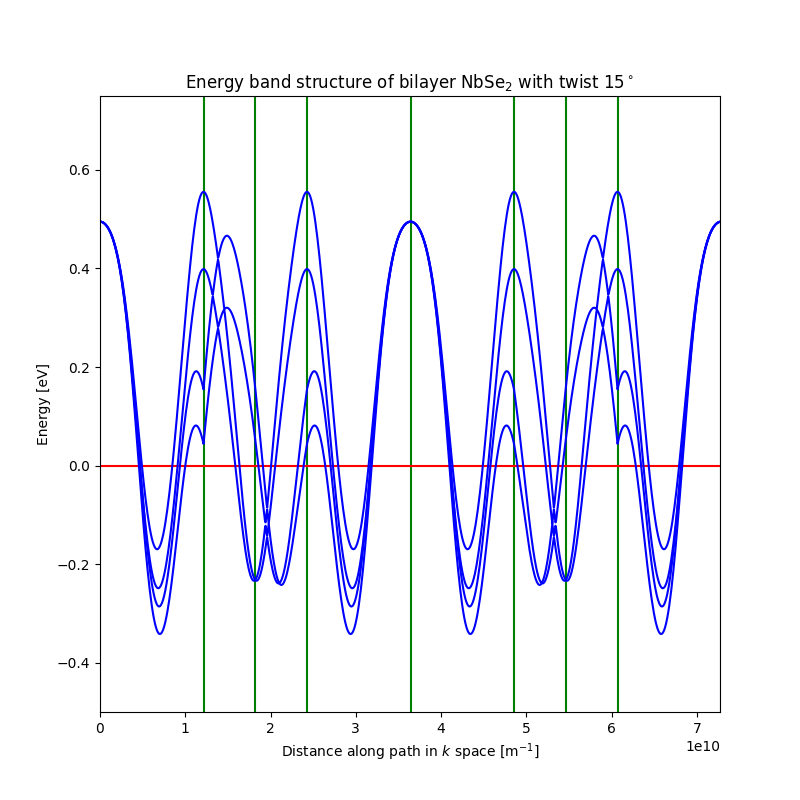
\includegraphics{heterostructure_evalues.png}}
    \caption{The four lowest energy eigenvalues of the heterostructure with a twist of 15$^\circ$ applied to the second layer. This plot is taken in the path $\Gamma \rightarrow \Gamma \rightarrow \Gamma$. For now, we are only looking at these eigenstates because they have energy near the Fermi level, and the corresponding Fermi-surface will describe the electronic properties of the material. The other eigenvalues are still computed.}
  \end{figure}
\end{frame}

\begin{frame}{Varying the angle}{Constructing a heterostructure}
  \begin{itemize}
    \item Animation of eigenvalues at varying angles (PDF).
    \item Notice that the intersection of energy bands varies with the angle of rotation.
    \item This will become very important in our work next semester when we apply perturbation theory to a model of coupled layers.
  \end{itemize}
\end{frame}

\begin{frame}{Coupling layers - the $d_{z^2}$ orbital}{What's next}
  \begin{itemize}
    \item Currently, we are assuming no interaction between the electronic states on different layers.

    \item Looking at the $d$ orbitals that we're modelling with the TBM, the $d_{z^2}$ orbital actually projects out (substantially) in the $z$ axis. It is therefore a good candidate for describing at inter-layer coupling effects.
  \end{itemize}

  \begin{figure}
    \centering
    \resizebox{4cm}{!}{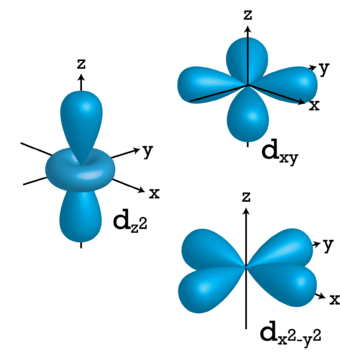
\includegraphics{d_orbitals.png}}
    \caption{Depictions of the $d$ orbitals from lumenlearning.com$^{[6]}$, note the projection of the $d_{z^2}$ orbital into the $z$ axis.}
  \end{figure}
\end{frame}

\begin{frame}{Naive steps forwards}{What's next}
  \begin{itemize}
    \item We will make several assumptions regarding the interaction of orbitals between layers. Firstly, that the influence of the $d_{xy}$ and $d_{x^2-y^2}$ orbitals is restricted to their corresponding $xy$ planes i.e. their own layers.

    \item This leaves the $d_{z^2}$ orbital. There is no quantum process that will allow for the transition into states of different spin.

    \item{So we are left with four processes to consider

      \begin{enumerate}
        \item $d_{z^2, \downarrow, 1} \rightarrow d_{z^2, \downarrow, 2}$
        \item $d_{z^2, \downarrow, 2} \rightarrow d_{z^2, \downarrow, 1}$
        \item $d_{z^2, \uparrow, 1} \rightarrow d_{z^2, \uparrow, 2}$
        \item $d_{z^2, \uparrow, 2} \rightarrow d_{z^2, \uparrow, 1}$
      \end{enumerate}

      where $d_{z^2, s, i}$ is the $d_{z^2}$ orbital with spin $s$ on layer $i$ (we take $i=2$ as the rotated layer).
      }

    \item All of these processes should have the same transition energy, the next step is to try and model them.
  \end{itemize}
\end{frame}

\begin{frame}{Coupling and the Hamiltonian}{What's next}
  \begin{itemize}
    \item{Previously our 12 by 12 heterostructure Hamiltonian was block diagonal, where each 6 by 6 block corresponded to one of the layers.
      \begin{equation}
        \hat{H}(\boldsymbol{k})=\left(\begin{array}{cc}
          \hat{H_1}(\boldsymbol{k}) & 0\\
          0 & \hat{H_2}(\boldsymbol{k'})
        \end{array}\right)
      \end{equation}
      }

    \item To account for the coupling we will add terms in the 0 blocks at positions that correspond to the four $d_{z^2}$ orbital transitions that we are interested in.

    \item{This will give us the modified Hamiltonian
      \begin{equation}
        \hat{H}(\boldsymbol{k})=\left(\begin{array}{cc}
          \hat{H_1}(\boldsymbol{k}) & T\\
          T^{\dagger} & \hat{H_2}(\boldsymbol{k'})
        \end{array}\right)
      \end{equation}

      Where $T$ is a 6 by 6 matrix containing our coupling term at (col, row) = (1,1) and (4,4); see the eigenvector. The nature of this coupling term $t(k, \theta)$ we are yet to determine.
      }
  \end{itemize}
\end{frame}

\begin{frame}{Coupling}{What's next}
  \begin{itemize}
    \item We construct a 'toy model' where we will set the coupling term in $T$ to be a constant. For now we have chosen 0.3 eV, just to see what the effect could look like on our band structure.
  \end{itemize}

  \begin{figure}
    \centering
    \resizebox{6cm}{!}{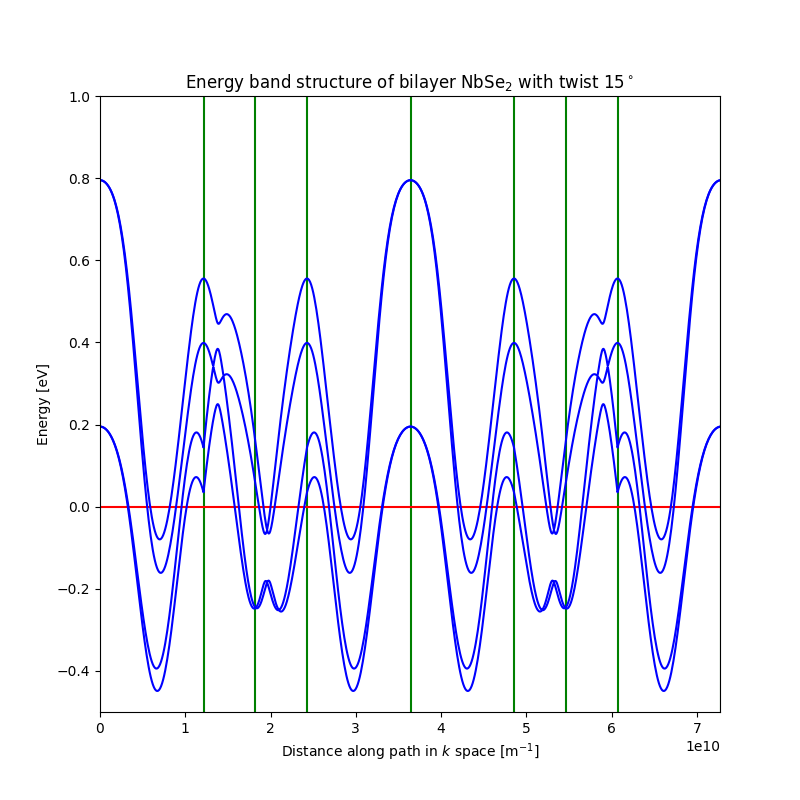
\includegraphics{coupled_heterostructure_evalues.png}}
    \caption{The four lowest energy eigenvalues of the heterostructure with a twist of 15$^\circ$ applied to the second layer. The 'toy model' coupling term is applied, there is a resulting effect on the electron bands that were previously unaffected by rotation.}
  \end{figure}
\end{frame}

\begin{frame}{Flattening bands}{What's next}
  \begin{itemize}
    \item Our coupling terms in our more complex heterostructure Hamiltonian will naturally result in a splitting of energy levels at degenerate eigenvalues as a consequence of perturbation theory.

    \item The previous graph manages to naively predict the splitting of energy levels at $\Gamma$.

    \item A consequence of this is that electron bands become "flatter" that is, they have a lower bandwidth.

    \item This results in a higher density of states at certain energy levels, with lower transition energies between them.

    \item Things get especially interesting when this flattening happens around the Fermi level, and will be the focus of our work going into the next semester.
  \end{itemize}
\end{frame}

\begin{frame}{References}
  \begin{enumerate}
    \item Cao, Y., Fatemi, V., Fang, S. et al, 2018. Unconventional superconductivity in magic-angle graphene superlattices. \textit{Nature}, 556, pp.43–50. DOI: 10.1038/nature26160.
    \item Bistritzer, R. MacDonald, A. H., 2011. Moiré bands in twisted double-layer graphene. \textit{Proceedings of the National Academy of Sciences}, 108(30), pp.12233-12237. DOI: 10.1073/pnas.1108174108
    \item Geim, A., Grigorieva, I., 2013. Van der Waals heterostructures. \textit{Nature}, 499, pp.419–425. DOI: doi.org/10.1038/nature12385.
    \item Freedman, D. H., 2019. With a Simple Twist, a ‘Magic’ Material Is Now the Big Thing in Physics. \textit{Quanta magazine} [Online]. Available from: https://www.quantamagazine.org/how-twisted-graphene-became-the-big-thing-in-physics-20190430/ [Accessed 13 December 2021].
    \item Habara, R. Wakabayashi, K., 2021. Optically induced spin current in monolayer ${\mathrm{NbSe}}_{2}$. \textit{PhysRevB}, 103(16), L161410. DOI: 10.1103/PhysRevB.103.L161410.
    \item  Orbitals, 2021. \textit{Lumen Chemistry for Non-Majors} [Online]. Available from: https://courses.lumenlearning.com/cheminter/chapter/orbitals/ [Accessed 13 December 2021].
  \end{enumerate}
\end{frame}

\end{document}
